\markboth{Battery Composition}{Battery Composition}
\section{Battery Composition}
The battery pack is modelled using a variation of the Composite design pattern with multiple composite classes\footnote{The basic Composite design pattern has one component interface, one composite class and one leaf class.}. This way, cells can be combined flexibly in various different topologies.

\subsection{Overview}
The \mcode{batteryInterface} is the abstract component that defines the interface for all objects in the composition. It is subclassed by all other battery elements. The \mcode{batteryCell} objects are the "leaves" and a composite can be one of the following classes:
\begin{itemize}
	\item \mcode{parallelElement}: A set of components in parallel.
	\item \mcode{seriesElementAE}: A set of components in series with active equalization.
	\item \mcode{seriesElementPE}: A set of components in series with passive equalization.
\end{itemize}
Each component can either be another composite object or a leaf.
\begin{figure}[b!]
	\captionsetup{type=figure}
	\centering
	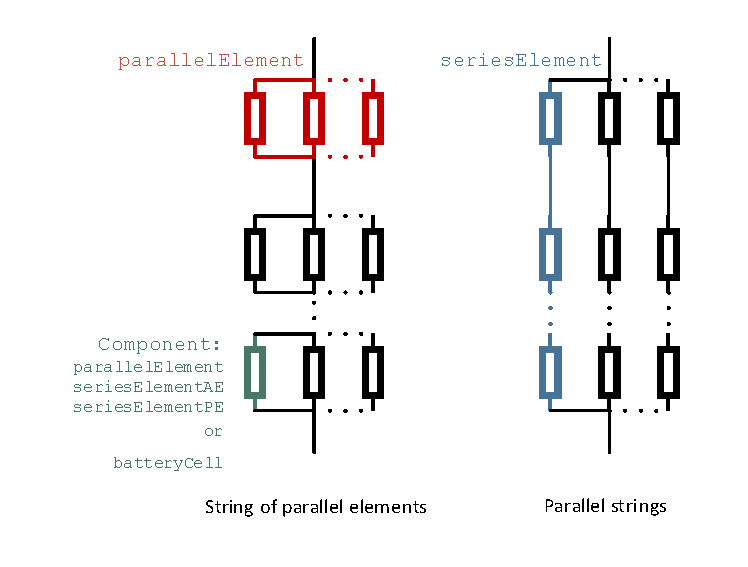
\includegraphics[width=\textwidth]{topologies2.pdf}
	\caption[Visualization of the possible battery topology compositions]{Visualization of the possible battery topology compositions.}
	\label{fig:topologies2}
\end{figure}
Figure~\ref{fig:topologies2} provides a visual overview of the topologies that are possible using different compositions. Using this variation of the Composite design pattern, the components can be combined in any possible way at runtime. The most common battery topologies are strings of parallel elements (SP) and parallel strings of cells (PS)~\cite{cordoba-arenas_control-oriented_2015}. In Figure~\ref{fig:topologies2}, these would be the case if all of the components (marked green) were cells. However, since every component can be either a cell or another composite, more complicated topologies are made possible in this package. \\
\begin{figure}[t!]
	\captionsetup{type=figure}
	\centering
	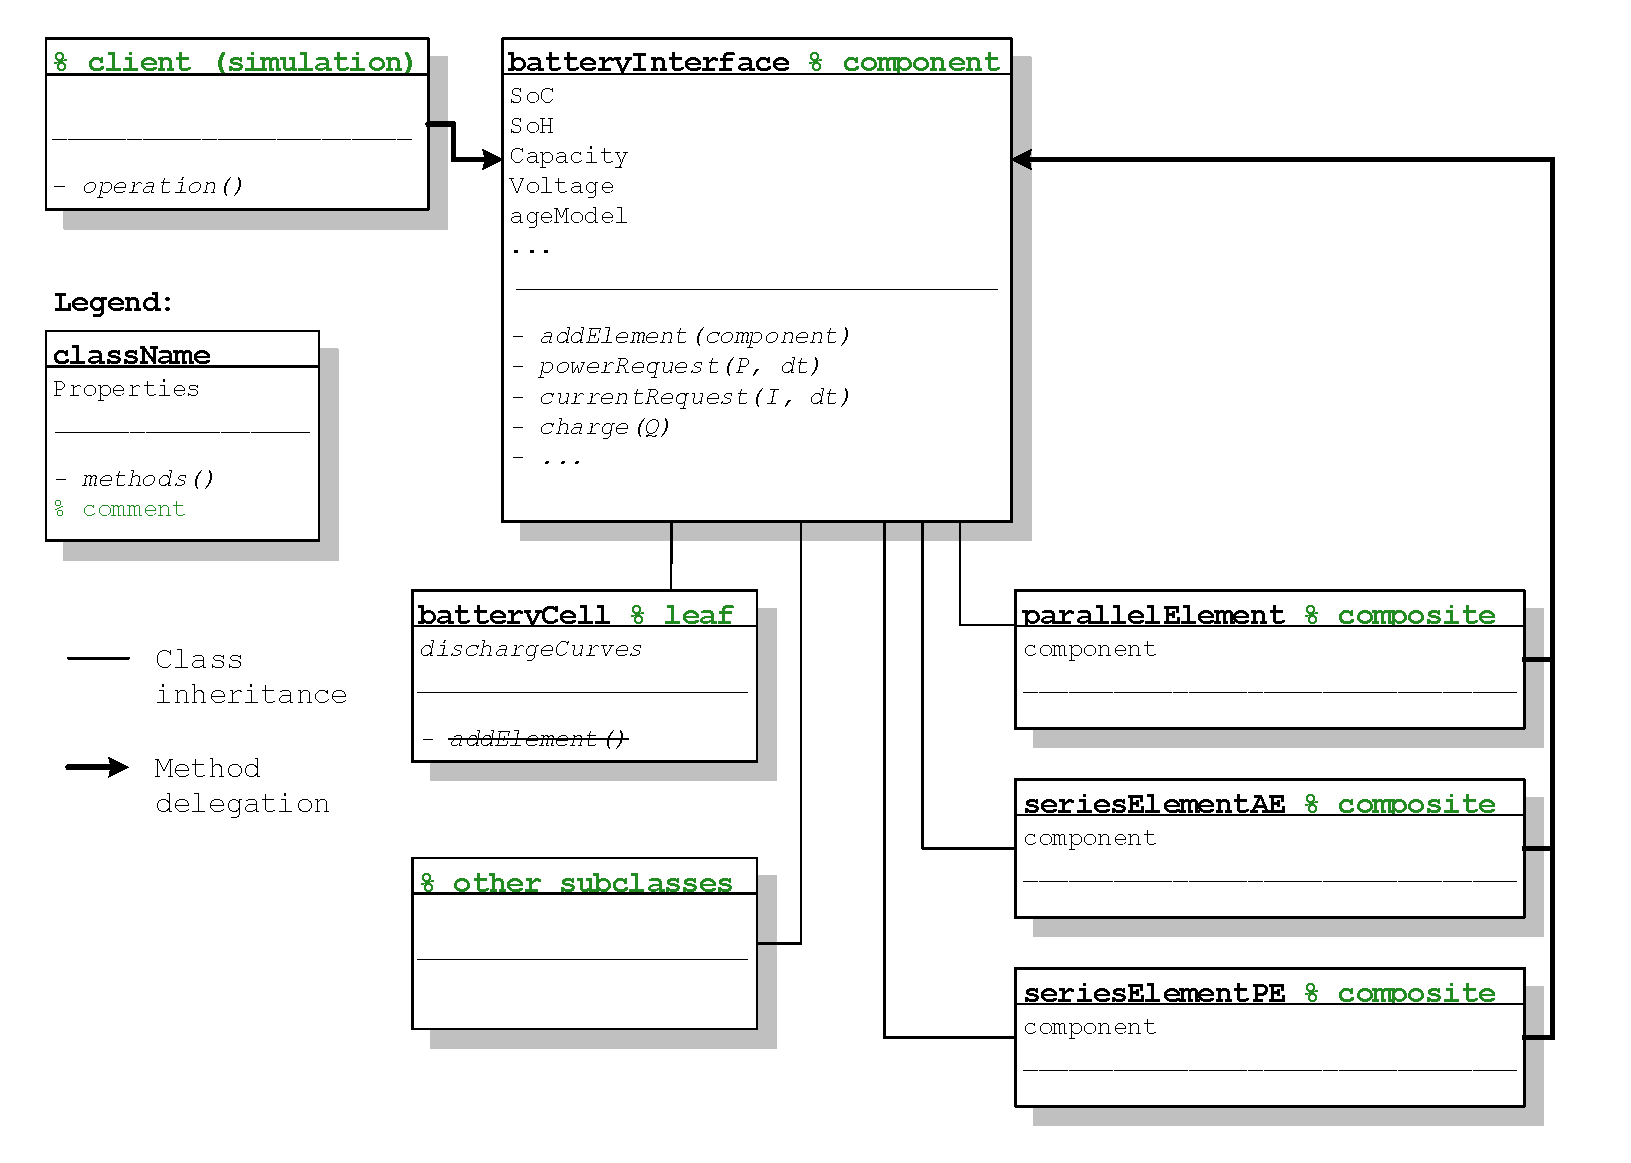
\includegraphics[width=\textwidth]{composite_schema.pdf}
	\caption[Class diagram of the battery composition with communication flows and inheritance links]{Class diagram of the battery composition with communication flows and inheritance links.}
	\label{fig:composite_schema}
\end{figure}

\subsection{Method delegation}
A pattern diagram of the classes used for the topology composition is depicted in Figure~\ref{fig:composite_schema}. Every composite element holds a reference to a component and delegates the methods called on it to said component. The delegated methods are wrapped with the rules of the respective topology, in a similar fashion as is done with the Decorator design pattern. An example of the method delegation for a PS configuration - a \mcode{parallelElement} that holds a set of \mcode{seriesElements}, each in turn holding a set of \mcode{batteryCells} objects - is visualized in Figure~\ref{fig:method_delegation}. In this example, a current \mcode{I} and the simulation time step size is passed to the \mcode{parallelElement} via a \mcode{getVoltage()} method. The \mcode{parallelElement} determines which portion of \mcode{I} to send to each of it's components and delegates the method. Each \mcode{seriesElement} does the same and delegates the method to it's \mcode{batteryCell} objects. These return their voltages back to the \mcode{seriesElements}, which sum up the results received from their cells and pass the sum back to the \mcode{parallelElement}. Finally, the \mcode{parallelElement} calculates the mean of all the summed up voltages it reveived and passes the end-result back to the client.
\begin{figure}[t!]
	\captionsetup{type=figure}
	\centering
	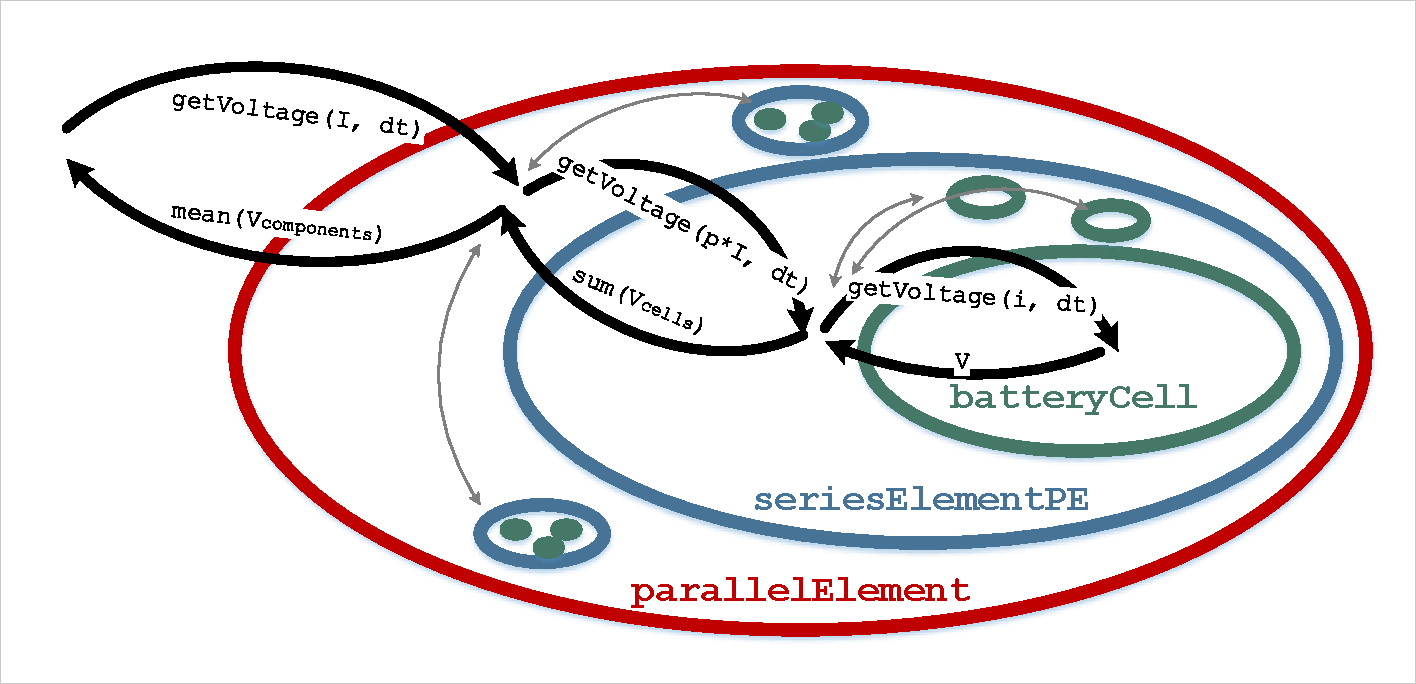
\includegraphics[width=\textwidth]{method_delegation.pdf}
	\caption[Example of a method being delegated across a battery pack composition]{Example of a method being delegated across a battery pack composition.}
	\label{fig:method_delegation}
\end{figure}
